\section{Frontend}

Frontend of an application is what consumers see at first and the way to interact with the middleware. The biggest challenge was designing interfaces for everyone and not only for developers. User experience is the key success of every applications. 

\subsection{Technologies}


\subsubsection{AngularJS}

AngularJS is now the leader for dynamic view in web-application. It is support by Google and private community. AngularJS strength is its two-way data binding. Whatever your are modifying, View or Model the other is updated instantly. However, the model stay the single-source-of-truth for the application state. AngularJS provide a high-level module to interact with RESTFul server called \emph{\$resource} and every CRUD function are defined easily like the following for the Action Target:

\begin{lstlisting}
iFluxFrontServices.factory('ActionTarget', ['$resource',
    function ($resource) {
        return $resource(baseUrl + '/actionTargets/:actionTargetId', {}, {
            query: {method: 'GET', isArray: true},
            save: {method: 'POST'},
            update: {method: 'PATCH', params: {actionTargetId: '@actionTargetId'}},
            get: {method: 'GET', params: {actionTargetId: '@actionTargetId'}},
            delete: {method: 'DELETE', params: {actionTargetId: '@actionTargetId'}}
        });
    }
]);
\end{lstlisting}

Some functionalities does not exists in core AngularJS, however the community has developed some plugins that was required to enhance the user experience. Here is a small list used in the project:
\begin{itemize}
  \item \textbf{Angular ui-ace} \url{https://github.com/angular-ui/ui-ace} Ace is an embeddable code editor and this plugin adapt Ace for Angular.
  \item \textbf{Angular ui-select} \url{https://github.com/angular-ui/ui-select} More than a dropdown list, it allow search, select and multi-select. 
  \item \textbf{Angular schema-form} \url{https://github.com/Textalk/angular-schema-form} The most usefull components that allow users to create forms based on JSON schema in Event Source Template and Action Target Template. The result is displayed in the instance (Event Source, Action Target) editor.    
\end{itemize}

\subsubsection{Jade}
What is Jade? \emph{Jade is a high performance template engine heavily influenced by Haml and implemented with JavaScript for node and browsers.} In iFlux, Jade is used to create Angular partials because HTML is verbose. 

Jade code for managing Organization in iFlux
\begin{lstlisting}
.container
    #page-content-wrapper
        h1 iFLUX Organization
        .big-panel
            .col-lg-12.form-horizontal
                .col-lg-6
                    h3 General Info
                    .form-group
                        label.col-sm-4.control-label(for='NameTemplate') email address
                        .col-sm-8
                            input#NameTemplate.form-control(name='nameTemplate', type='email', placeholder='email address', ng-model='form.email', required='')
        .col-lg-12
            .buttonbar
                a.btn.btn-primary(ng-click='cancel()') Cancel
                a.btn.btn-success(ng-click='submitForm()') Add user
\end{lstlisting}

Transformation in HTML
\begin{lstlisting}
<div class="container">
  <div id="page-content-wrapper">
    <h1>iFLUX Organization</h1>
    <div class="big-panel">
      <div class="col-lg-12 form-horizontal">
        <div class="col-lg-6">
          <h3>General Info</h3>
          <div class="form-group">
            <label for="NameTemplate" class="col-sm-4 control-label">email address</label>
            <div class="col-sm-8">
              <input id="NameTemplate" name="nameTemplate" type="email" placeholder="email address" ng-model="form.email" required="" class="form-control"/>
            </div>
          </div>
        </div>
      </div>
    </div>
    <div class="col-lg-12">
      <div class="buttonbar"><a ng-click="cancel()" class="btn btn-primary">Cancel</a><a ng-click="submitForm()" class="btn btn-success">Add user</a></div>
    </div>
  </div>
</div>
\end{lstlisting}




\subsubsection{Stylus}

Write CSS directly is not anymore done by web developers. CSS preprocessor technologies like Saas LESS or Stylus replace it and allow you to use variables, nesting, inheritance, mixins, importing, etc. Stylus is different from the two others by omitting brackets, colons and semi-colons in your code. The result of the preprocessor is a standard CSS file.

Example of a contextual selector with Stylus
\begin{lstlisting}
.panel
  height auto
  margin 0 auto

  .panel-green
    border-color light-green

  .panel-red
    border-color light-red

  .panel-info
    border-color blue-help
\end{lstlisting}

The result after compilation
\begin{lstlisting}
.panel {
    height: auto;
    margin: 0 auto;
}
.panel .panel-green {
    border-color: #cfc;
}
.panel .panel-red {
    border-color: #fdd;
}
.panel .panel-info {
    border-color: #bce8f1;
}
\end{lstlisting} 

\subsubsection{Grunt and Bower}
Grunt is a JavaScript task runner and allow you to define repetitive task and automate it, like compile Stylus, run the web server, process Jade, etc. We define a watch task that process Stylus file after each modification and integrates it on the running website. With that, your website has always the latest modifications. With the command \emph{grunt} in shell, the webserver start, compile Stylus and run the watch task. 

The watch task in Gruntfile.js
\begin{lstlisting}
grunt.initConfig({
  pkg: grunt.file.readJSON('package.json'),
  develop: {
    server: {
      file: 'app.js'
    }
  },
  stylus: {
    dist: {
      files: {
        'public/css/style.css': 'public/css/style.styl'
      }
    }
  },
  watch: {
    options: {
      nospawn: true,
      livereload: reloadPort
    },
    js: {
      files: [
        'app.js',
        'app/**/*.js',
        'config/*.js'
      ],
      tasks: ['develop', 'delayed-livereload']
    },
    css: {
      files: [
        'public/css/*.styl'
      ],
      tasks: ['stylus'],
      options: {
        livereload: reloadPort
      }
    },
    views: {
      files: [
        'app/views/*.jade',
        'app/views/**/*.jade'
      ],
      options: { livereload: reloadPort }
    }
  }
});
\end{lstlisting}

Bower is a package manager for the web stack. You define in \emph{bower.json} which version of your components you want and it installed your package. Here is the dependencies of the frontend. There are lots of Angular modules provided by Angular or by users on Github. 

\begin{lstlisting}
{
  "name": "code",
  "version": "0.0.1",
  "ignore": [e
    "**/.*",
    "node_modules",
    "components"
  ],
  "private": true,
  "dependencies": {
    "angular": "~1.4.1",
    "angular-bootstrap": "~0.13.0",
    "angular-bootstrap-switch": "~0.4.1",
    "angular-mocks": "1.4.1",
    "angular-route": "~1.4.1",
    "angular-resource": "~1.4.1",
    "angular-sanitize": "~1.4.1",
    "angular-schema-form": "~0.8.2",
    "angular-ui-ace": "~0.2.3",
    "angular-ui-select": "~0.12.0",
    "bootstrap": "3.3.x",
    "fontawesome": "~4.3.0",
    "jquery": "~2.1.1",
    "ngstorage": "~0.3.6",
    "jquery-ui": "~1.10.4"
  },
  "resolutions": {
    "angular": "1.4.1"
  }
}
\end{lstlisting}

By calling \emph{bower install} every dependencies will be downloaded and installed. To install a new dependency, type \emph{bower install --save package-name}. The dependency will be installed and the file bower.json will be updated with the new entry. 

\subsection{UX design}
The masterpiece of UX design is a responsive website with bootstrap technology. We did not develop the frontend for a mobile because of the complexity of interfaces. Mobile phone are not useful when you have to write JS expression, navigate to find the help or fill long form. However, the website is responsive for the different resolution of the screen. 

The concept of CRUD function is applied to the interface which for every parts of the model, has a management interface and an editor/view interface. In the management view, you can create, read, update or delete an entry. We did not innovate for the presentation. 

\subsubsection{Event Source}
On the Event Source Template editor we employed the project \emph{Angular Schema Form} \url{http://schemaform.io/} which allow you to create a dynamic Angular form based on the JSON Schema. To instantiate an event source the user have to provide a certain amount of data and he will do that through the dynamic form. It is the keystone of the frontend to configure dynamically distant objects or services. 

An example of Json schema and the result form generated in figure \ref{fig:iflux-event-source-form}. 
\begin{lstlisting}
{
	"$schema": "http://json-schema.org/draft-04/schema#",
	"type": "object",
	"properties": {
		"all": {
			"type": "boolean"
		},
		"default": {
			"type": "boolean"
		},
		"zipCodes": {
			"type": "array",
			"minItems": 1,
			"items": {
				"type": "integer"
			},
			"uniqueItems": true
		}
	}
}
\end{lstlisting}

The form is displayed with the default UI which is the following code. You can modify the visual aspect of the form by adding: placeholder, button, organize the form with Tab, change the checkbox into radio button, ... 
\begin{lstlisting}
["*"]
\end{lstlisting}

\begin{figure}
\centering
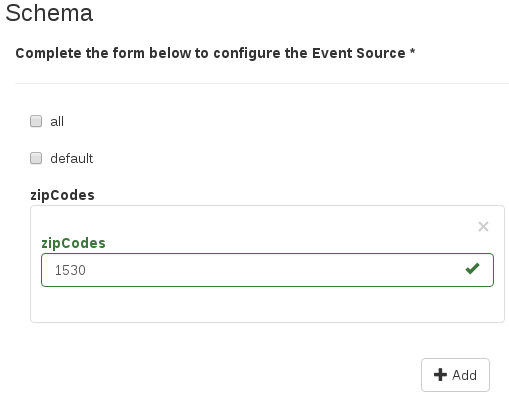
\includegraphics[width=0.8\columnwidth]{figures/event-source-form.png}
\caption{Event Sources form}
\label{fig:iflux-event-source-form}
\end{figure}


The figure \ref{fig:iflux-event-source} is the management interface for Event Source Template and Event Source. 
\begin{figure}
\centering
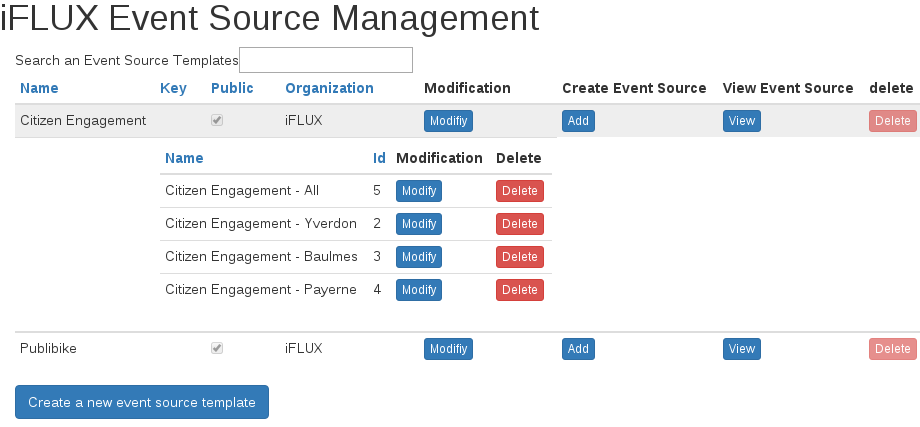
\includegraphics[width=1\columnwidth]{figures/eventSource.png}
\caption{Event Sources management}
\label{fig:iflux-event-source}
\end{figure}

\subsubsection{Action Target}

The Action Target interface is almost the same than Event Source. \emph{Angular Schema Form} is also used to define endpoints and configure them. 

\subsubsection{Rules}
To create a rules, you have to define a minimum of one condition and one action. Of course, you can add as much as you want. Configure a rules is not an easy task. This is why modal views are bind to dropdown lists to help users to choose the right instance or the right action/event type. To write JS expression, a help box displays properties of the event based on the chosen event type. The figure\ref{fig:iflux-rules-action} below show an action box with the help - a part of the rules form. Javascript editor is based on \emph{Ace} which is an online code editor. It provide syntax highlighting, automatic indent, live syntax checker, etc. We make it resizable to allow a better visibility of your function. The code below is for one editor box. Lots of options are available, like autocompletion, code snippets, type of code, ...
\begin{lstlisting}
.js-editor-medium(resizable='')
    div(required='', name='conditionExpression', ui-ace="{
    	require: ['ace/ext/language_tools'],\
       		advanced: {\
   	   		enableSnippets: true,\
       			enableBasicAutocompletion: true,\
       			enableLiveAutocompletion: true\
       		}, useWrapMode : true,  showGutter: true,  theme:'monokai',  mode: 'javascript',onChange: schemaChanged}", 
   		ng-model='condition.fn.expression')
\end{lstlisting}

\begin{figure*}
\centering
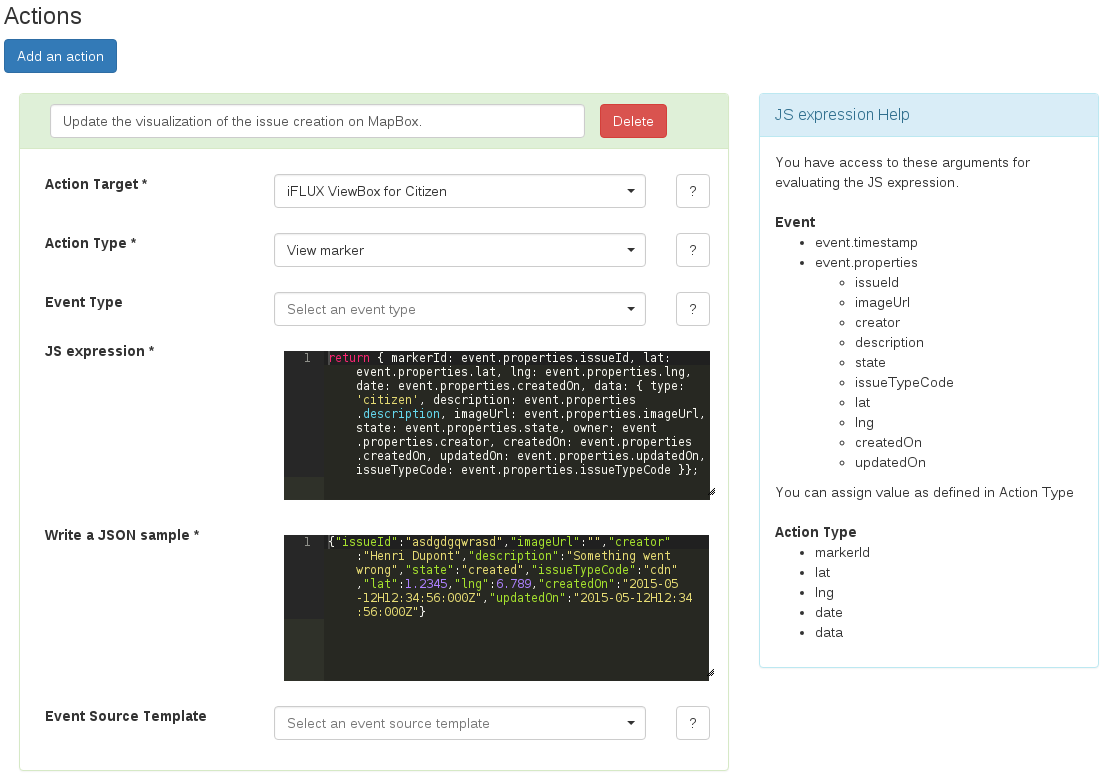
\includegraphics[width=0.9\textwidth]{figures/rules-transformation.png}
\caption{Rules editor - one action}
\label{fig:iflux-rules-action}
\end{figure*}
